\documentclass{beamer}

\usetheme{Torino}
\AtBeginSection[] 
{ 
  \begin{frame}<beamer> 
    \frametitle{Agenda} 
    \tableofcontents[currentsection] 
  \end{frame} 
}  % for recurrent Agenda slide
\numberwithin{equation}{section} % Number equations with sections



\usepackage{amsmath}
\usepackage{amsfonts}
\usepackage[latin1]{inputenc}
\usepackage{amsmath}
\usepackage{amsfonts}
\usepackage{amssymb}
\usepackage{makeidx}
\usepackage{tabularx}
\usepackage{url}
\usepackage[toc,acronym,description]{glossaries}
\usepackage{cite}
\usepackage{hyperref}
\usepackage[noend,boxed,fillcomment]{algorithm2e}
\usepackage{multicol}
\usepackage{fancyvrb}
\usepackage{color}
\usepackage{subfigure}
\usepackage{graphicx}
\usepackage{pdfpages}
% use \usepackage[pdfborder=0in]{hyperref} instead to disable red box links
%\usepackage[T1]{fontenc}
\newcommand{\BibTeX}{{\sc Bib}\TeX}
\newcommand{\rischintegrate}{\texttt{risch\_integrate()}}
\hyphenation{Sym-Py an-ti-der-iv-a-tive an-ti-der-iv-a-tives
an-ti-diff-er-en-tia-tion Goo-gle arc-trig-o-no-met-ric
non-el-e-men-tary}
\makeatletter
\def\PY@reset{\let\PY@it=\relax \let\PY@bf=\relax%
    \let\PY@ul=\relax \let\PY@tc=\relax%
    \let\PY@bc=\relax \let\PY@ff=\relax}
\def\PY@tok#1{\csname PY@tok@#1\endcsname}
\def\PY@toks#1+{\ifx\relax#1\empty\else%
    \PY@tok{#1}\expandafter\PY@toks\fi}
\def\PY@do#1{\PY@bc{\PY@tc{\PY@ul{%
    \PY@it{\PY@bf{\PY@ff{#1}}}}}}}
\def\PY#1#2{\PY@reset\PY@toks#1+\relax+\PY@do{#2}}

\def\PY@tok@gd{\def\PY@tc##1{\textcolor[rgb]{0.63,0.00,0.00}{##1}}}
\def\PY@tok@gu{\let\PY@bf=\textbf\def\PY@tc##1{\textcolor[rgb]{0.50,0.00,0.50}{##1}}}
\def\PY@tok@gt{\def\PY@tc##1{\textcolor[rgb]{0.00,0.25,0.82}{##1}}}
\def\PY@tok@gs{\let\PY@bf=\textbf}
\def\PY@tok@gr{\def\PY@tc##1{\textcolor[rgb]{1.00,0.00,0.00}{##1}}}
\def\PY@tok@cm{\let\PY@it=\textit\def\PY@tc##1{\textcolor[rgb]{0.25,0.50,0.50}{##1}}}
\def\PY@tok@vg{\def\PY@tc##1{\textcolor[rgb]{0.10,0.09,0.49}{##1}}}
\def\PY@tok@m{\def\PY@tc##1{\textcolor[rgb]{0.40,0.40,0.40}{##1}}}
\def\PY@tok@mh{\def\PY@tc##1{\textcolor[rgb]{0.40,0.40,0.40}{##1}}}
\def\PY@tok@go{\def\PY@tc##1{\textcolor[rgb]{0.50,0.50,0.50}{##1}}}
\def\PY@tok@ge{\let\PY@it=\textit}
\def\PY@tok@vc{\def\PY@tc##1{\textcolor[rgb]{0.10,0.09,0.49}{##1}}}
\def\PY@tok@il{\def\PY@tc##1{\textcolor[rgb]{0.40,0.40,0.40}{##1}}}
\def\PY@tok@cs{\let\PY@it=\textit\def\PY@tc##1{\textcolor[rgb]{0.25,0.50,0.50}{##1}}}
\def\PY@tok@cp{\def\PY@tc##1{\textcolor[rgb]{0.74,0.48,0.00}{##1}}}
\def\PY@tok@gi{\def\PY@tc##1{\textcolor[rgb]{0.00,0.63,0.00}{##1}}}
\def\PY@tok@gh{\let\PY@bf=\textbf\def\PY@tc##1{\textcolor[rgb]{0.00,0.00,0.50}{##1}}}
\def\PY@tok@ni{\let\PY@bf=\textbf\def\PY@tc##1{\textcolor[rgb]{0.60,0.60,0.60}{##1}}}
\def\PY@tok@nl{\def\PY@tc##1{\textcolor[rgb]{0.63,0.63,0.00}{##1}}}
\def\PY@tok@nn{\let\PY@bf=\textbf\def\PY@tc##1{\textcolor[rgb]{0.00,0.00,1.00}{##1}}}
\def\PY@tok@no{\def\PY@tc##1{\textcolor[rgb]{0.53,0.00,0.00}{##1}}}
\def\PY@tok@na{\def\PY@tc##1{\textcolor[rgb]{0.49,0.56,0.16}{##1}}}
\def\PY@tok@nb{\def\PY@tc##1{\textcolor[rgb]{0.00,0.50,0.00}{##1}}}
\def\PY@tok@nc{\let\PY@bf=\textbf\def\PY@tc##1{\textcolor[rgb]{0.00,0.00,1.00}{##1}}}
\def\PY@tok@nd{\def\PY@tc##1{\textcolor[rgb]{0.67,0.13,1.00}{##1}}}
\def\PY@tok@ne{\let\PY@bf=\textbf\def\PY@tc##1{\textcolor[rgb]{0.82,0.25,0.23}{##1}}}
\def\PY@tok@nf{\def\PY@tc##1{\textcolor[rgb]{0.00,0.00,1.00}{##1}}}
\def\PY@tok@si{\let\PY@bf=\textbf\def\PY@tc##1{\textcolor[rgb]{0.73,0.40,0.53}{##1}}}
\def\PY@tok@s2{\def\PY@tc##1{\textcolor[rgb]{0.73,0.13,0.13}{##1}}}
\def\PY@tok@vi{\def\PY@tc##1{\textcolor[rgb]{0.10,0.09,0.49}{##1}}}
\def\PY@tok@nt{\let\PY@bf=\textbf\def\PY@tc##1{\textcolor[rgb]{0.00,0.50,0.00}{##1}}}
\def\PY@tok@nv{\def\PY@tc##1{\textcolor[rgb]{0.10,0.09,0.49}{##1}}}
\def\PY@tok@s1{\def\PY@tc##1{\textcolor[rgb]{0.73,0.13,0.13}{##1}}}
\def\PY@tok@sh{\def\PY@tc##1{\textcolor[rgb]{0.73,0.13,0.13}{##1}}}
\def\PY@tok@sc{\def\PY@tc##1{\textcolor[rgb]{0.73,0.13,0.13}{##1}}}
\def\PY@tok@sx{\def\PY@tc##1{\textcolor[rgb]{0.00,0.50,0.00}{##1}}}
\def\PY@tok@bp{\def\PY@tc##1{\textcolor[rgb]{0.00,0.50,0.00}{##1}}}
\def\PY@tok@c1{\let\PY@it=\textit\def\PY@tc##1{\textcolor[rgb]{0.25,0.50,0.50}{##1}}}
\def\PY@tok@kc{\let\PY@bf=\textbf\def\PY@tc##1{\textcolor[rgb]{0.00,0.50,0.00}{##1}}}
\def\PY@tok@c{\let\PY@it=\textit\def\PY@tc##1{\textcolor[rgb]{0.25,0.50,0.50}{##1}}}
\def\PY@tok@mf{\def\PY@tc##1{\textcolor[rgb]{0.40,0.40,0.40}{##1}}}
\def\PY@tok@err{\def\PY@bc##1{\fcolorbox[rgb]{1.00,0.00,0.00}{1,1,1}{##1}}}
\def\PY@tok@kd{\let\PY@bf=\textbf\def\PY@tc##1{\textcolor[rgb]{0.00,0.50,0.00}{##1}}}
\def\PY@tok@ss{\def\PY@tc##1{\textcolor[rgb]{0.10,0.09,0.49}{##1}}}
\def\PY@tok@sr{\def\PY@tc##1{\textcolor[rgb]{0.73,0.40,0.53}{##1}}}
\def\PY@tok@mo{\def\PY@tc##1{\textcolor[rgb]{0.40,0.40,0.40}{##1}}}
\def\PY@tok@kn{\let\PY@bf=\textbf\def\PY@tc##1{\textcolor[rgb]{0.00,0.50,0.00}{##1}}}
\def\PY@tok@mi{\def\PY@tc##1{\textcolor[rgb]{0.40,0.40,0.40}{##1}}}
\def\PY@tok@gp{\let\PY@bf=\textbf\def\PY@tc##1{\textcolor[rgb]{0.00,0.00,0.50}{##1}}}
\def\PY@tok@o{\def\PY@tc##1{\textcolor[rgb]{0.40,0.40,0.40}{##1}}}
\def\PY@tok@kr{\let\PY@bf=\textbf\def\PY@tc##1{\textcolor[rgb]{0.00,0.50,0.00}{##1}}}
\def\PY@tok@s{\def\PY@tc##1{\textcolor[rgb]{0.73,0.13,0.13}{##1}}}
\def\PY@tok@kp{\def\PY@tc##1{\textcolor[rgb]{0.00,0.50,0.00}{##1}}}
\def\PY@tok@w{\def\PY@tc##1{\textcolor[rgb]{0.73,0.73,0.73}{##1}}}
\def\PY@tok@kt{\def\PY@tc##1{\textcolor[rgb]{0.69,0.00,0.25}{##1}}}
\def\PY@tok@ow{\let\PY@bf=\textbf\def\PY@tc##1{\textcolor[rgb]{0.67,0.13,1.00}{##1}}}
\def\PY@tok@sb{\def\PY@tc##1{\textcolor[rgb]{0.73,0.13,0.13}{##1}}}
\def\PY@tok@k{\let\PY@bf=\textbf\def\PY@tc##1{\textcolor[rgb]{0.00,0.50,0.00}{##1}}}
\def\PY@tok@se{\let\PY@bf=\textbf\def\PY@tc##1{\textcolor[rgb]{0.73,0.40,0.13}{##1}}}
\def\PY@tok@sd{\let\PY@it=\textit\def\PY@tc##1{\textcolor[rgb]{0.73,0.13,0.13}{##1}}}

\def\PYZbs{\char`\\}
\def\PYZus{\char`\_}
\def\PYZob{\char`\{}
\def\PYZcb{\char`\}}
\def\PYZca{\char`\^}
% for compatibility with earlier versions
\def\PYZat{@}
\def\PYZlb{[}
\def\PYZrb{]}
\makeatother


\title{Report on the Risch Algorithm for Symbolic
Integration and Implementation in the SymPy Computer Algebra System}
\author{Aaron Meurer}
\date{December 10, 2010}

\begin{document}

\begin{frame}
    \titlepage
\end{frame}

\begin{frame} 
    \frametitle{Agenda} 
    \tableofcontents 
\end{frame} 

\section{Background}
\subsection{Definitions}

\begin{frame}
    \frametitle{Definitions}
    \begin{itemize}
        \item {\bf Integration} 
        \begin{itemize}
            \item One of two fundamental operations in calculus (the other
            being differentiation).
            \item Informally, $\int_a^b{f(x)\,dx}$ represents the area under
            the curve defined by the function $f(x)$ from the points $x=a$
            to $x=b$.
            \item The Fundamental Theorem of Calculus states that
            integration and antidifferentiation, the inverse operation of
            differentiation, are essentially the same thing.
            \end{itemize}
    \pause
        \item {\bf Algebraic}
        \begin{itemize}
            \item A function is algebraic if it is the root of a polynomial
            with coefficients that are rational functions with rational
            number coefficients.  
            \item For example, the function $\sqrt{x + 1}$ is algebraic
            because it is the root of the polynomial $y^2 = x + 1$. 
        \end{itemize}
    \end{itemize}
\end{frame}

\begin{frame}
    \frametitle{Definitions}
    \begin{itemize}
        \item {\bf Transcendental}
        \begin{itemize}
            \item A function is transcendental if it is not algebraic.  
            \item A function is \textit{purely transcendental} if it does
            not contain any algebraic components.  
            \item $e^x$, $\ln{x}$, $\sin{x}$, $\cos{x}$, and $\tan{x}$ are
            all transcendental.  
            \item Roughly speaking, a function is transcendental if it
            contains one of these, and it is purely transcendental if it
            does not contain any radicals.
            \begin{itemize}
                \item $e^{x + 1}$ is purely transcendental
                \item $\sqrt[3]{\ln{x}}$ is transcendental but not
                purely transcendental
                \item $\sqrt{x}$ is neither transcendental nor purely
                transcendental (it is algebraic)
            \end{itemize}
        \end{itemize}
    \end{itemize}
\end{frame}

\begin{frame}
    \frametitle{Definitions}
    \begin{itemize}
        \item {\bf Elementary}
        \begin{itemize}
            \item Roughly speaking, a function is elementary if it can
            be represented as a combination of exponentials, logarithms,
            powers, and trigonometric functions by addition,
            subtraction, multiplication, division, and composition. 
            \item For example, $\frac{\sin{(x^2 +
            1)}}{\sqrt[3]{\ln{x}}}$ is elementary, but
            $\frac{2}{\sqrt{\pi}}\int{e^{-x^2}\,dx}$, the error
            function, is not.
        \end{itemize}
    \end{itemize}
\end{frame}

\section{The Risch Algorithm}

\subsection{Liouville's Theorem}

\begin{frame}
    \frametitle{Liouville's Theorem}
    \begin{itemize}
        \item If a function $f$ has an elementary integral, then the
        integral can always be written in the form
        \begin{equation}
            \label{liouville's theorem}
            \int{f} = v + \sum_{n=1}^m{c_i\ln{u_i}}
        \end{equation}
        where $v$ and the $u_i$ are ``parts'' of $f$, and the $c_i$ are
        constants.
        \pause
        \item In other words, if we can show that $\int{f}$ does not
        have this form, then we have shown that it is not elementary.
    \end{itemize}
\end{frame}

\subsection{The Transcendental Risch Algorithm}

\begin{frame}
    \frametitle{The Transcendental Risch Algorithm}
    \begin{itemize}
        \item First we must parse the expression
        \item Make sure it is purely transcendental
        \begin{itemize}
            \item e.g., $e^{\frac{1}{2}\ln{x}}$ is NOT transcendental
            because it is equivalent to $\sqrt{x}$
        \end{itemize}
    \pause
    \item Break the function into transcendental ``levels''
    \item For example, for $e^{\tan{x^2}}$, we have $e^{\tan{x^2}}$,
    then $\tan{x^2}$, then $x$.
    \pause
    \item Integrate starting at the top until out integral only has
    lower levels
    \item Then recursively integrate
    \item When we reach $x$ (always the lowest ``level''), we are done
    \end{itemize}
\end{frame}

\begin{frame}
    \frametitle{The Transcendental Risch Algorithm}
    \begin{itemize}
        \item Four steps, each which breaks up the integral into a
        smaller integral and part of the solution
        \begin{equation}
        \label{smaller integral}
        \int{f(x)\,dx} = p(x) + \int{q(x)\,dx}
        \end{equation}
        \pause
        \item The steps are 
            \begin{enumerate}
                \item Hermite Reduction
                \item Polynomial Reduction
                \item Residue Criterion: Computes the logarithmic part
                (the $c_i$ and $u_i$)
                \item We then get a ``polynomial'' in our top level
                function
            \end{enumerate}
            \pause
            \begin{itemize}
                \item Each case reduces to a subproblem
                    \begin{itemize}
                        \item Exponential Case $\longrightarrow$ Risch
                        Differential Equation
                        \item Primitive (Logarithmic) Case
                        $\longrightarrow$ Parametric Risch Differential
                        Equation
                        \item Tangent Case $\longrightarrow$ Coupled
                        Risch Differential Equation
                    \end{itemize}
            \end{itemize}
    \pause
    \item Steps 3 and 4 potentially prove that the integral is nonelementary
    \end{itemize}
\end{frame}

\subsubsection{Example: Risch Differential Equation}

\begin{frame}
    \frametitle{Example: Risch Differential Equation}
    \pause
    \begin{equation}
    \label{exponential integral}
    \int{p(x)e^{q(x)}\,dx}
    \end{equation}
    is equivalent to 
    \begin{equation}
    \label{rischde}
    y' + fy = g
    \end{equation}
    having a solution $y$, where $f$ and $g$ come directly from $p(x)$
    and $q(x)$
    \pause
    \begin{itemize}
        \item Liouville's Theorem implies $y$ must have only ``parts''
        from $f$ and $g$.
        \pause
        \item Complex, case-by-case algorithm to solve \ref{rischde}
        \pause
        \item If it finds that no solution can not exist, then it has shown
        that \ref{exponential integral} is not elementary.
    \end{itemize}
\end{frame}

\section{Implementation in SymPy}

\begin{frame}
    \frametitle{Implementation in SymPy}
    \begin{figure}
    \subfigure{
\includegraphics[width=.32\textwidth]{python-logo-master-v3-TM.png}}
    \subfigure{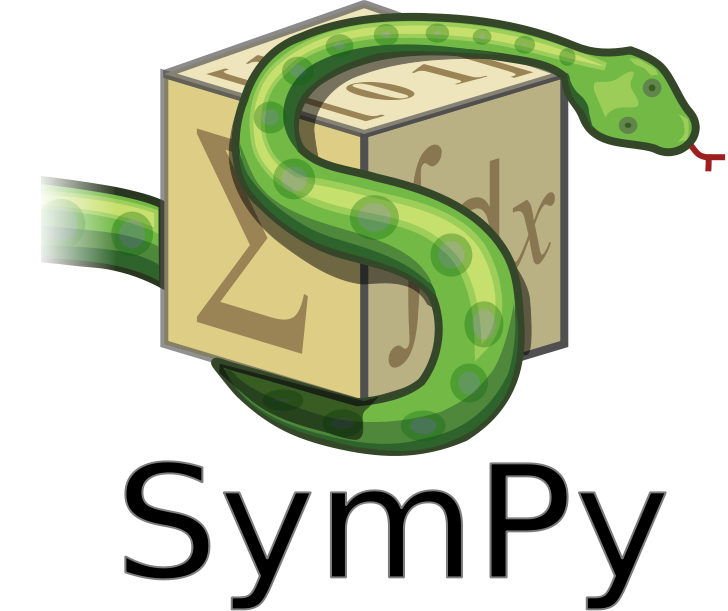
\includegraphics[width=.32\textwidth]{sympy.png}}
   \subfigure{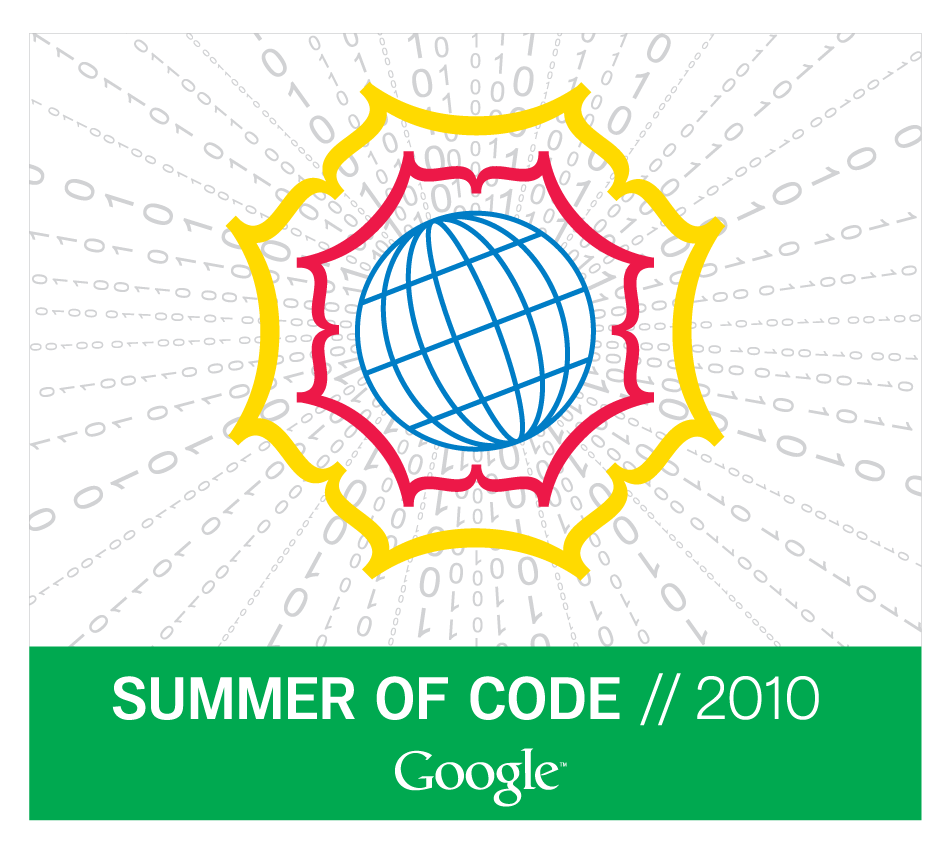
\includegraphics[width=.32\textwidth]{GSoC_2010_logo/2010_NoURL_950x846px.png}}
   \end{figure}
    Over the summer of 2010, I worked for the Python Software
    Organization with the SymPy project under the Google Summer of Code
    program to implement the transcendental Risch Algorithm in SymPy.
\end{frame}

\begin{frame}
    \frametitle{Implementation in SymPy}
    \begin{itemize}
        \item End result: \rischintegrate{} function
        \pause
        \item Orders of magnitude faster than old \texttt{integrate()} function
        \item Able to solve much more
        \item And it can prove that integrals are nonelementary!
    \end{itemize}
\end{frame}
\begin{frame}
    \frametitle{Implementation in SymPy}
    \begin{figure}[t!]
        \subfigure{\raisebox{1in}{\includegraphics[width=.481\textwidth]{algorithmfull}}}
        \subfigure{\includegraphics[width=.5\textwidth]{polyrischdenocancel2full.pdf}}
    \end{figure}
%    \begin{figure}
%        \subfigure{\begin{algorithm}[H]
    \SetCommentSty{textrm}
    \SetFillComment
    \dontprintsemicolon
%    \TitleOfAlgo{{\bf PolyRischDENoCancel2}($b$, $c$, $D$, $n$)}
%    \SetAlgorithmName{{\bf PolyRischDENoCancel2}($b$, $c$, $D$, $n$)}
    {\bf PolyRischDENoCancel2}($b$, $c$, $D$, $n$)
    \tcc*[f]{Poly Risch d.e. -- no cancellation}\;
    \BlankLine
    \Indp
%    \tcc*[f]{Poly Risch d.e. -- no cancellation}}\;
    \BlankLine
    \tcc*[f]{Given a derivation $D$ on $k[t]$, $n$ either an integer or
    $+\infty$, and $b, c\in k[t]$ with $\mathrm{deg}(b)< \delta(t) - 1$
    and either $D = d/dt$ or $\delta(t) \geq 2$, return either ``no
    solution'', in which case the equation $Dq + bq = c$ has no solution
    of degree at most $n$ in $k[t]$, or a solution $q \in k[t]$ of this
    equation with $\mathrm{deg}(q) \leq n$, or the tuple $(h, b_0, c_0)$
    such that $h \in k[t]$, $b_0,c_0\in k[t]$, and for any solution
    $q\in k[t]$ of degree at most $n$ of $Dq + bq = c$, $y = q - h$ is a
    solution in $k$ of $Dy + b_0y=c_0$.}\;
    \BlankLine
    $q \leftarrow 0$\;
    \While{$c\neq 0$}{
        \lIf{$n=0$}{$m\leftarrow 0$} \lElse{$m\leftarrow \mathrm{deg}(c)
        = \delta(t) + 1$}\;
        \lIf{$n < 0$ or $m < 0$ or $m > n$}{\Return ``no solution''}\;
        \lIf{$m > 0$}{$p\leftarrow (\mathrm{lc}(c)/(m\lambda(t)))t^m$}\;
        \Else(\tcc*[f]{$m =  0$}){
            \lIf{$\mathrm{deg}(b) \neq \mathrm{deg}(c)$}{\Return ``no
            solution''}\;
            \lIf{$\mathrm{deg}(b) = 0$}{\Return $(q, c, b)$}\;
            $p \leftarrow \mathrm{lc}(c)/\mathrm{lc}(b)$\;
        }
        $q \leftarrow q + p$\;
        $n \leftarrow m - 1$\;
        $c \leftarrow c - Dp - bp$\;
    }
    \Return $q$
\end{algorithm}}
%        \subfigure{\input{../report/polyrischdenocancel2}}
%    \end{figure}
\end{frame}

\begin{frame}
    \frametitle{Implementation in SymPy}
    \begin{figure}
    \begin{flushleft}
    \subfigure{\includegraphics[width=.7\textwidth]{../report/sample1.pdf}}
    \subfigure{\includegraphics[width=.7\textwidth]{../report/sample2.pdf}}
    \pause
    \subfigure{\includegraphics[width=.7\textwidth]{../report/sample3.pdf}}
    \subfigure{\includegraphics[width=.7\textwidth]{../report/sample4.pdf}}
    \end{flushleft}
    \end{figure}
\end{frame}

\begin{frame}
    \frametitle{Implementation in SymPy}
    \begin{figure}
    \begin{flushleft}
    \subfigure{\includegraphics[width=.7\textwidth]{../report/sample5.pdf}}
    \subfigure{\includegraphics[width=.7\textwidth]{../report/sample7.pdf}}
    \subfigure{\includegraphics[width=.7\textwidth]{../report/sample10.pdf}}
    \subfigure{\includegraphics[width=.7\textwidth]{../report/sample11.pdf}}
    \end{flushleft}
    \end{figure}
\end{frame}

\begin{frame}
    \frametitle{Implementation in SymPy}
    Let's look at how long it takes to compute $\int{x^{10}e^x\,dx}$ and $\int{x^{20}e^x\,dx}$.
    \begin{figure}
    \begin{flushleft}
    \subfigure{\includegraphics[width=.7\textwidth]{../report/sample14.pdf}}
    \subfigure{\includegraphics[width=.7\textwidth]{../report/sample15.pdf}}
    \subfigure{\includegraphics[width=.7\textwidth]{../report/sample16.pdf}}
    \subfigure{\includegraphics[width=.7\textwidth]{../report/sample17.pdf}}
    \end{flushleft}
    \end{figure}
    (\texttt{integrate()} is the old function and \rischintegrate{} is
    the new function)\\
    \pause
    {\bf The new implementation is both orders of magnitude faster, and
    asymptotically faster!}
\end{frame}

\begin{frame}
    \begin{itemize}
        \item All of SymPy (including my work) is open source (BSD license)
        \item You can download SymPy at \url{www.sympy.org}
        \item My development branch is at
        \url{www.github.com/asmeurer/sympy/tree/integration3} (it
        isn't merged into the main repo yet)
    \end{itemize}
\end{frame}

\section{Questions}

\begin{frame}
    \frametitle{Questions?}
    \huge{Questions?}
\end{frame}

\end{document}
